% Vilnius University beamer template
% Created in 2024 by Joana Katina
% Adapted for TurtleBot3 room exploration presentation

\documentclass[12pt]{beamer}

\renewcommand{\figurename}{}
\renewcommand{\tablename}{}
\renewcommand\thefigure{\arabic{figure} pav.}
\renewcommand\thetable{\arabic{table} lentelė.}

\usepackage{graphicx}
\usepackage{listings}
\usepackage{algorithm,algorithmic}
\usepackage{caption}
\usepackage{subfig}
\usepackage{hyperref}
\usepackage{tikz}
\usetikzlibrary{positioning, arrows.meta, fit, backgrounds}

\usetheme{Madrid}

\title[]{Patalpos žemėlapio sudarymas naudojant TurtleBot Burger robotą}
\subtitle[]{Kursinis darbas}
\author[Gvidas Bačianskas, Denisas Savickis]{Gvidas Bačianskas, Denisas Savickis}
\date{}

%% Darbo vadovas
\addtobeamertemplate{author}{}{Darbo vadovas: prof. dr. Virginijus Marcinkevičius\par}

\setbeamertemplate{navigation symbols}{}
\titlegraphic{
\includegraphics[width=2cm]{resources/MIF.png}}

\usepackage{VUMIF}
\usepackage[T1]{fontenc}

\begin{document}

%% 1. Titulinis
\begin{frame}
    \titlepage
\end{frame}

%% 2. Įvadas
\begin{frame}{Įvadas}
    \textbf{Problema:}
    \begin{itemize}
        \item Autonominiai robotai turi gebėti suvokti aplinką ir priimti sprendimus be žmogaus įsikišimo
        \item Patalpų žemėlapio sudarymas kartu su lokalizacija (SLAM) yra pagrindas navigacijai
        \item Skirtingos tyrinėjimo strategijos lemia skirtingą efektyvumą
    \end{itemize}
    
    \vspace{0.5cm}
    \textbf{Darbo tikslas:}
    \begin{itemize}
        \item Išanalizuoti technologijas ir algoritmus, naudojamus robotų autonominiame tyrinėjime
        \item Realizuoti pasirinktus algoritmus naudojant TurtleBot3 Burger
        \item Palyginti algoritmų efektyvumą simuliacinėje ir realioje aplinkoje
    \end{itemize}
\end{frame}

%% 3. Uždaviniai
\begin{frame}{Darbo uždaviniai}
    \begin{enumerate}
        \item Atlikti literatūros analizę apie mobilių robotų navigaciją ir patalpų žemėlapių sudarymo algoritmus
        \item Sukonstruoti TurtleBot Burger robotą ir išmokti jį valdyti bei programuoti
        \item Realizuoti TurtleBot Burger simuliacinę aplinką
        \item Realizuoti pasirinktus autonominio tyrinėjimo algoritmus
        \item Atlikti eksperimentinius sistemos bandymus, renkant duomenis apie žemėlapio sudarymo laiką ir tikslumą
        \item Palyginti fizinio roboto ir simuliacinio modelio veikimo rezultatus
    \end{enumerate}
\end{frame}

%% 4. TurtleBot3 Burger
\begin{frame}{TurtleBot3 Burger platforma}
    \begin{columns}[onlytextwidth]
        \column{0.55\textwidth}
        \textbf{Pagrindiniai komponentai:}
        \begin{itemize}
            \item \textbf{Dynamixel XM430} -- varikliai su integruotais enkoderiais
            \item \textbf{OpenCR} -- žemo lygio mikrovaldiklis
            \item \textbf{Raspberry Pi 3} -- pagrindinis kompiuteris (ROS2, SLAM, navigacija)
            \item \textbf{LiDAR LDS-02} -- 360° lazerinis jutiklis (0,16--8 m diapazonas)
        \end{itemize}
        \column{0.45\textwidth}
        \begin{figure}
            \centering
            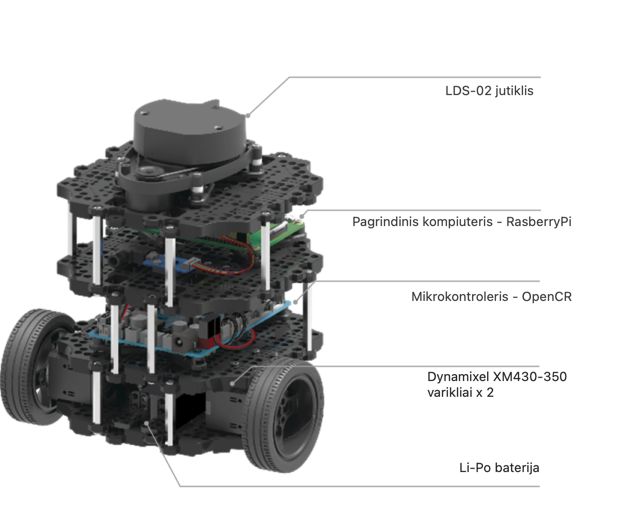
\includegraphics[width=0.95\textwidth]{images/TurtleBot.png}
            \caption{TurtleBot3 Burger}
        \end{figure}
    \end{columns}
\end{frame}

%% 5. Sistemos architektūra
\begin{frame}{Sistemos architektūra}
    \begin{columns}[onlytextwidth]
        \column{0.5\textwidth}
        \textbf{Dviejų lygių architektūra:}
        \begin{itemize}
            \item \textbf{Žemas lygis (OpenCR):}
            \begin{itemize}
                \item Variklių valdymas
                \item Odometrijos skaičiavimas
            \end{itemize}
            \item \textbf{Aukštas lygis (RPi + ROS2):}
            \begin{itemize}
                \item SLAM žemėlapio sudarymas
                \item Autonominio tyrinėjimo algoritmai
                \item Navigacijos planavimas
            \end{itemize}
        \end{itemize}
        \column{0.5\textwidth}
        \begin{figure}
            \centering
            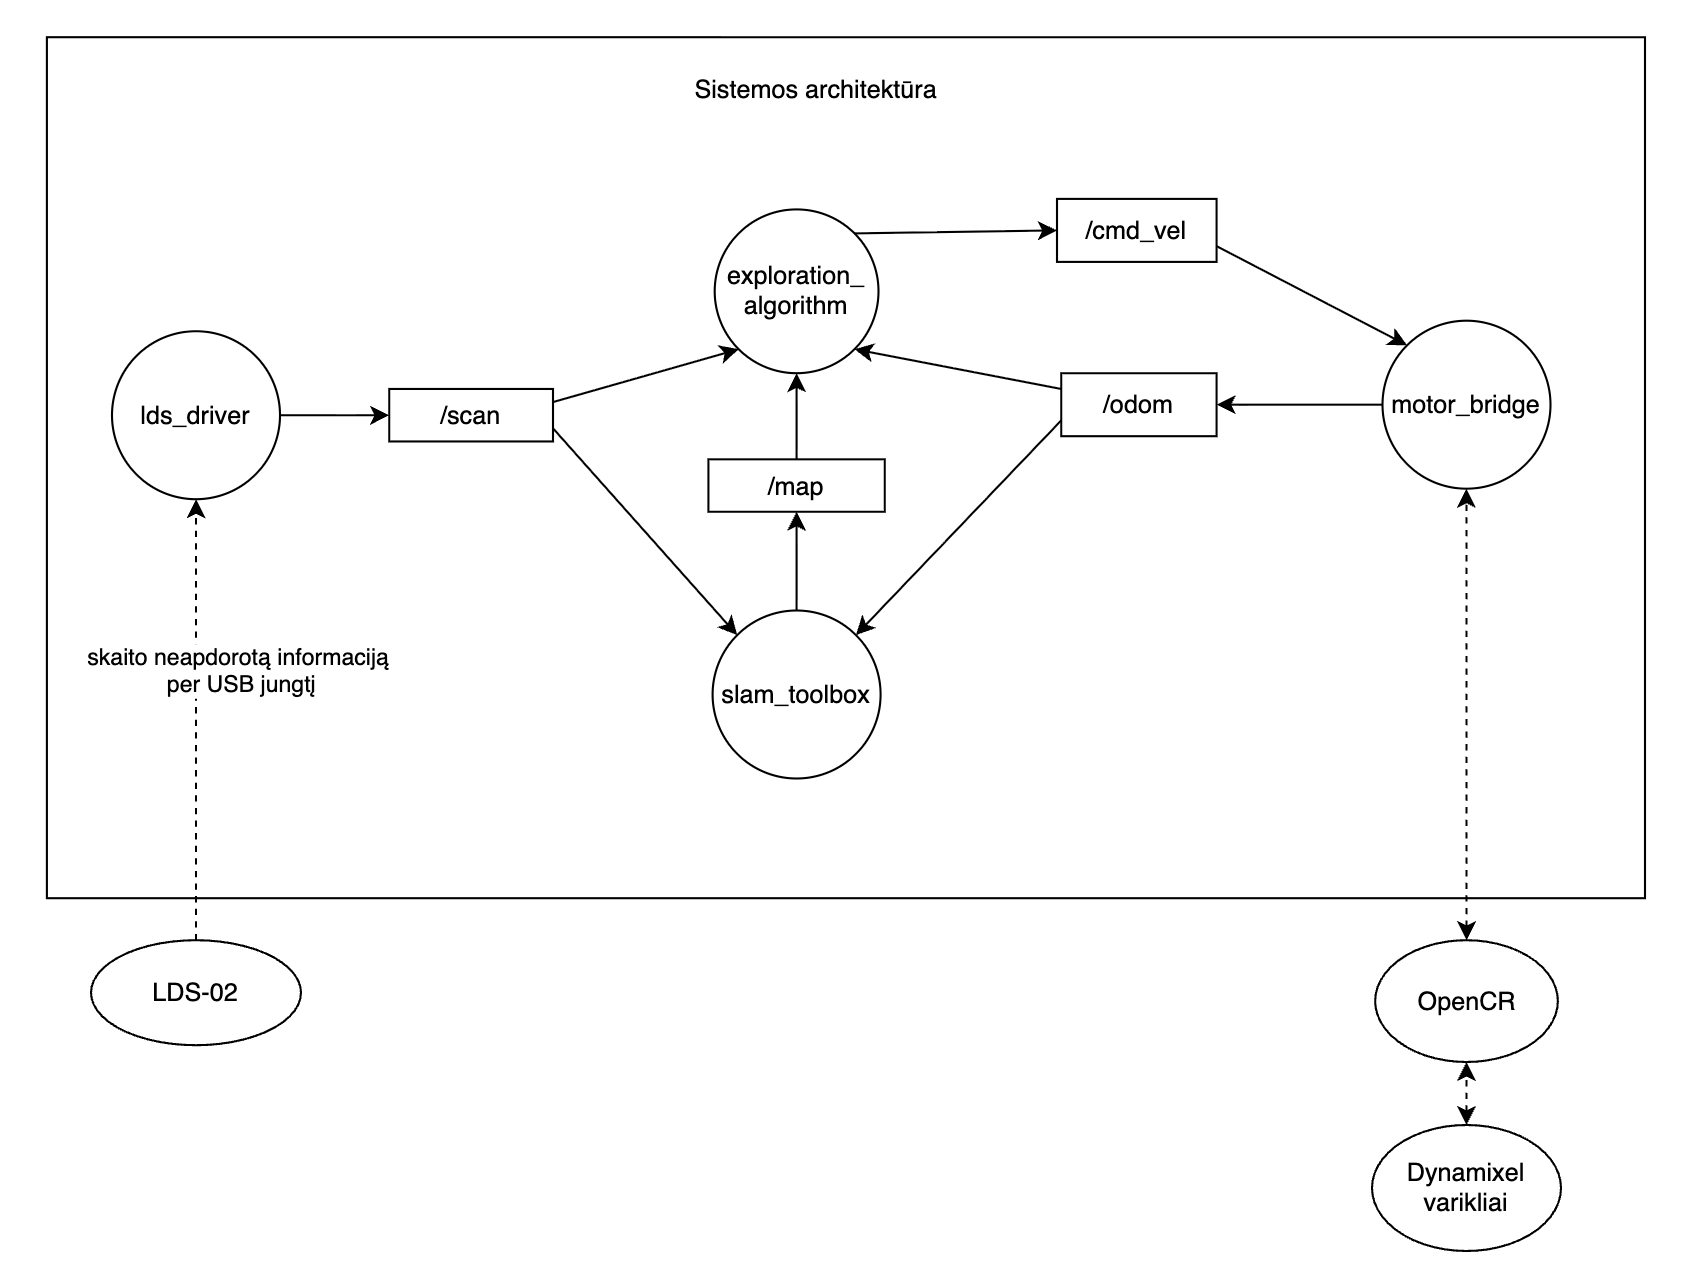
\includegraphics[width=1.1\textwidth]{images/roboto_sistemos_arch.png}
            \caption{Roboto sistemos architektūra}
        \end{figure}
    \end{columns}
\end{frame}

%% 6. SLAM ir navigacija
\begin{frame}{SLAM ir navigacija}
    \textbf{Užimtumo tinklas (Occupancy Grid):}
    \begin{itemize}
        \item Aplinka suskaidoma į langelius
        \item Kiekvienas langelis: \textbf{laisvas}, \textbf{užimtas}, \textbf{nežinomas}
    \end{itemize}
    
    \vspace{0.3cm}
    \textbf{Naudojami įrankiai:}
    \begin{itemize}
        \item \textbf{SLAM Toolbox} -- grafų optimizavimo SLAM algoritmas
        \begin{itemize}
            \item Efektyvus kilpų uždarymas
            \item Pastovus klaidų taisymas
        \end{itemize}
        \item \textbf{Navigacija} -- du skirtingi būdai:
        \begin{itemize}
            \item Frontier: Nav2 (kelių planavimas, costmap)
            \item BFS: tiesioginis variklių valdymas
        \end{itemize}
    \end{itemize}
\end{frame}

%% 10. Simuliacinė aplinka
\begin{frame}{Simuliacinė aplinka}
    \begin{columns}[onlytextwidth]
        \column{0.5\textwidth}
        \textbf{Gazebo simuliatorius:}
        \begin{itemize}
            \item Roboto, aplinkos, sensorių modeliavimas
            \item Fizikos modeliavimas
            \item Parametrai pritaikyti pagal realų robotą
        \end{itemize}
        
        \vspace{0.3cm}
        \textbf{Patalpos modelis:}
        \begin{itemize}
            \item 10x10 m patalpa
            \item Įvairaus dydžio kliūtys
        \end{itemize}
        \column{0.5\textwidth}
        \begin{figure}
            \centering
            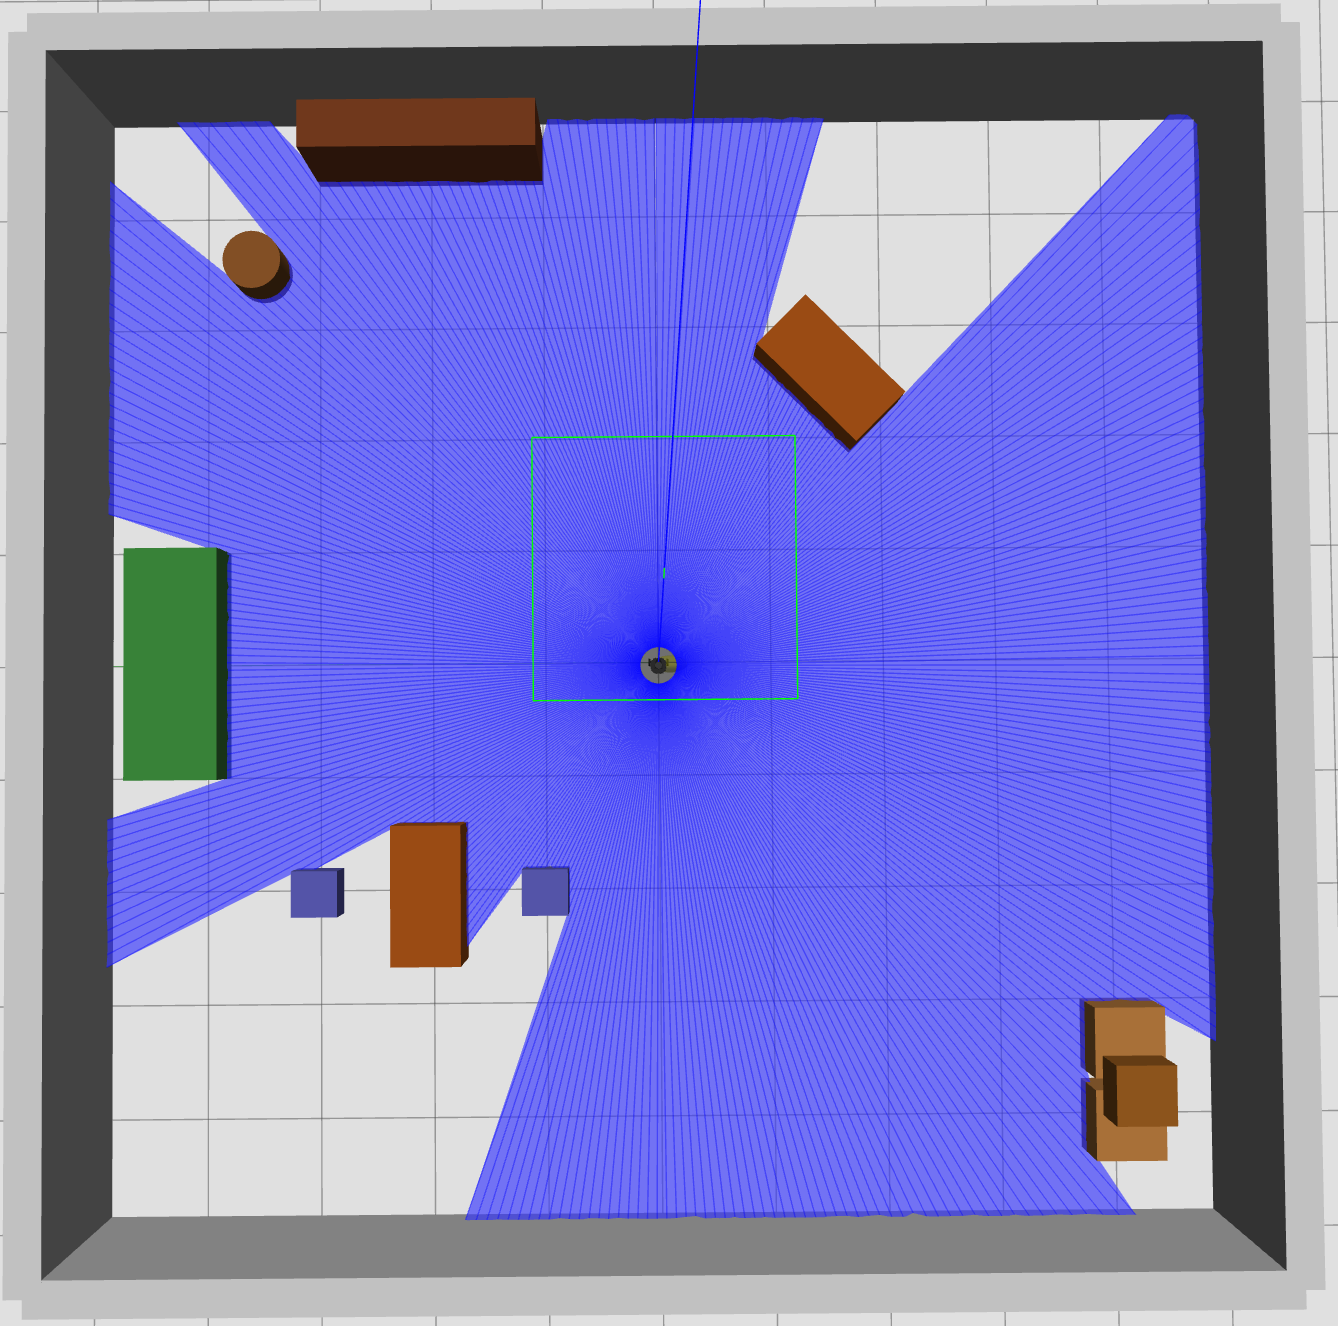
\includegraphics[width=0.95\textwidth]{images/medium_room.png}
            \caption{Simuliacinė patalpa}
        \end{figure}
    \end{columns}
\end{frame}

%% 9. Programinė architektūra
\begin{frame}{Programinė architektūra}
    \begin{center}
    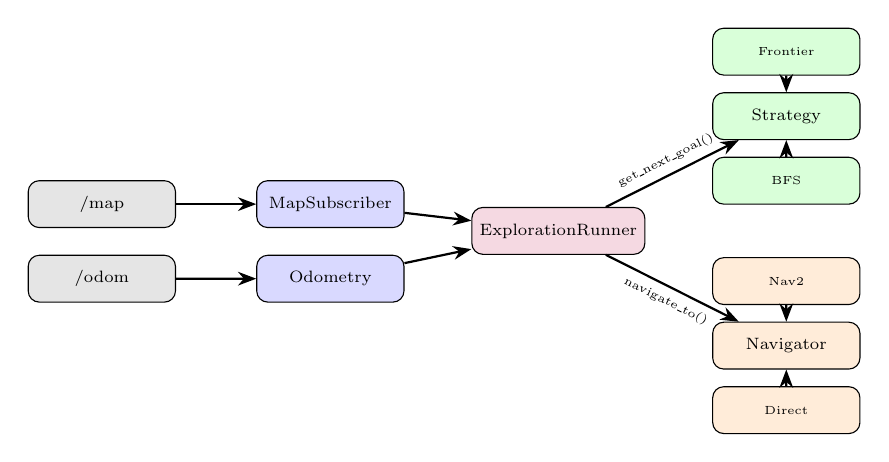
\begin{tikzpicture}[
        node distance=0.8cm and 1.2cm,
        box/.style={rectangle, draw, rounded corners, minimum width=2.2cm, minimum height=0.7cm, align=center, font=\scriptsize},
        rosbox/.style={box, fill=gray!20},
        corebox/.style={box, fill=blue!15},
        algobox/.style={box, fill=green!15},
        navbox/.style={box, fill=orange!15},
        runnerbox/.style={box, fill=purple!15},
        arrow/.style={-{Stealth}, thick},
        dataarrow/.style={arrow, dashed},
        scale=0.85, transform shape
    ]
        % ROS2 topics
        \node[rosbox] (map) {/map};
        \node[rosbox, below=0.4cm of map] (odom) {/odom};
        
        % Core
        \node[corebox, right=1.2cm of map] (mapsub) {MapSubscriber};
        \node[corebox, right=1.2cm of odom] (odometry) {Odometry};
        
        % Runner
        \node[runnerbox, right=1cm of mapsub, yshift=-0.4cm] (runner) {ExplorationRunner};
        
        % Strategy
        \node[algobox, above right=1cm and 1cm of runner] (strategy) {Strategy};
        \node[algobox, above=0.25cm of strategy, font=\tiny] (frontier) {Frontier};
        \node[algobox, below=0.25cm of strategy, font=\tiny] (bfs) {BFS};
        
        % Navigator
        \node[navbox, below right=1cm and 1cm of runner] (navigator) {Navigator};
        \node[navbox, above=0.25cm of navigator, font=\tiny] (nav2) {Nav2};
        \node[navbox, below=0.25cm of navigator, font=\tiny] (direct) {Direct};
        
        % Arrows
        \draw[arrow] (map) -- (mapsub);
        \draw[arrow] (odom) -- (odometry);
        \draw[arrow] (mapsub) -- (runner);
        \draw[arrow] (odometry) -- (runner);
        \draw[arrow] (runner) -- node[above, font=\tiny, sloped] {get\_next\_goal()} (strategy);
        \draw[arrow] (runner) -- node[below, font=\tiny, sloped] {navigate\_to()} (navigator);
        
        % Implementation arrows
        \draw[dataarrow] (frontier) -- (strategy);
        \draw[dataarrow] (bfs) -- (strategy);
        \draw[dataarrow] (nav2) -- (navigator);
        \draw[dataarrow] (direct) -- (navigator);
    \end{tikzpicture}
    \end{center}
    
    \vspace{0.2cm}
    \textbf{Strategijos šablonas:} lengvas algoritmų keitimas nekeičiant kitų dalių
\end{frame}

%% 7. Frontier algoritmas
\begin{frame}{Ribomis paremtas (Frontier) algoritmas}
    \textbf{Pagrindinė idėja:} Rasti ribas tarp ištirtų ir neištirtų zonų
    
    \vspace{0.3cm}
    \textbf{Ribų aptikimo žingsniai:}
    \begin{enumerate}
        \item Rasti laisvus langelius greta nežinomų 
        \item Pašalinti langelius šalia sienų
        \item Sugrupuoti į atskiras ribas
    \end{enumerate}
    
    \vspace{0.3cm}
    \textbf{Tikslo parinkimas:}
    \begin{itemize}
        \item Kiekvienai ribai suplanuojamas kelias per Nav2
        \item Pasirenkama riba su \textbf{trumpiausiu keliu}
        \item Nepasiekiamos ribos įtraukiamos į juodąjį sąrašą
    \end{itemize}
\end{frame}

%% 8. BFS algoritmas
\begin{frame}{BFS algoritmas su kainos vertinimu}
    \textbf{Pagrindinė idėja:} Kelio ieškojimas pločiu, vengiant artumo prie sienų
    
    \vspace{0.3cm}
    \textbf{Kelio planavimas:}
    \begin{itemize}
        \item Prioritetinė eilė
        \item Kaina: $C_{viso} = C_{atstumas} + C_{bauda}$
        \item Bauda didėja artėjant prie sienų $\rightarrow$ kelias eina patalpos viduriu
    \end{itemize}
    
    \vspace{0.3cm}
    \textbf{Saugumo mechanizmai:}
    \begin{itemize}
        \item \textbf{Avarinis stabdymas:} kliūtis $<$ 15,5 cm
        \item \textbf{Juodasis sąrašas:} nepasiekiami tikslai
        \item \textbf{Atsistatymo režimas:} atbulinė eiga + sukimasis
    \end{itemize}
\end{frame}

%% 11. Rezultatai: fizinis robotas
\begin{frame}{Rezultatai: fizinis robotas}
    \begin{table}
        \centering
        \begin{tabular}{|l|c|c|c|}
            \hline
            \textbf{Algoritmas} & \textbf{Laikas (s)} & \textbf{Atstumas (m)} & \textbf{Plotas (m²)} \\
            \hline
            Frontier & 60,1 & 0,32 & 1,52 \\
            \hline
            BFS & 85,2 & 1,06 & 1,59 \\
            \hline
        \end{tabular}
    \end{table}
    
    \begin{columns}[onlytextwidth]
        \column{0.5\textwidth}
        \begin{figure}
            \centering
            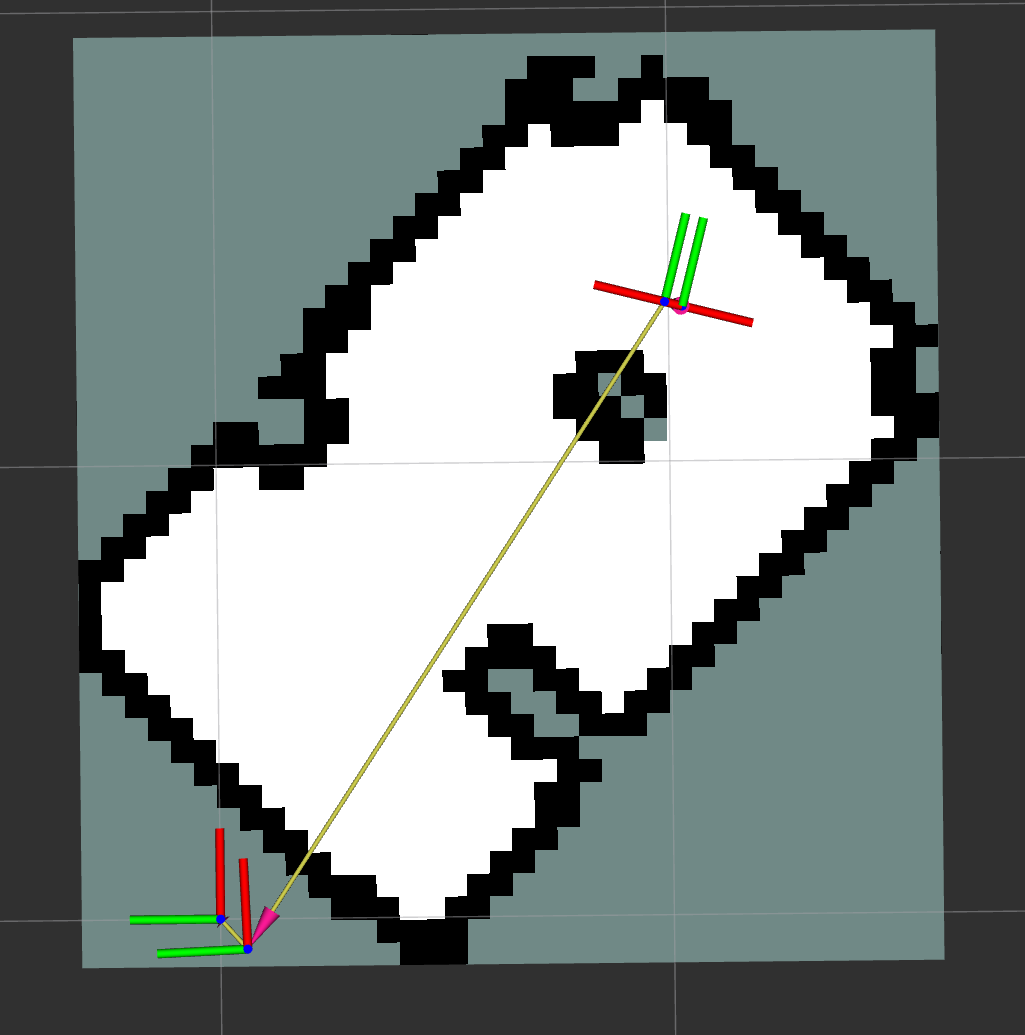
\includegraphics[width=0.8\textwidth]{images/frontier-real.png}
            \caption{Frontier žemėlapis}
        \end{figure}
        \column{0.5\textwidth}
        \begin{figure}
            \centering
            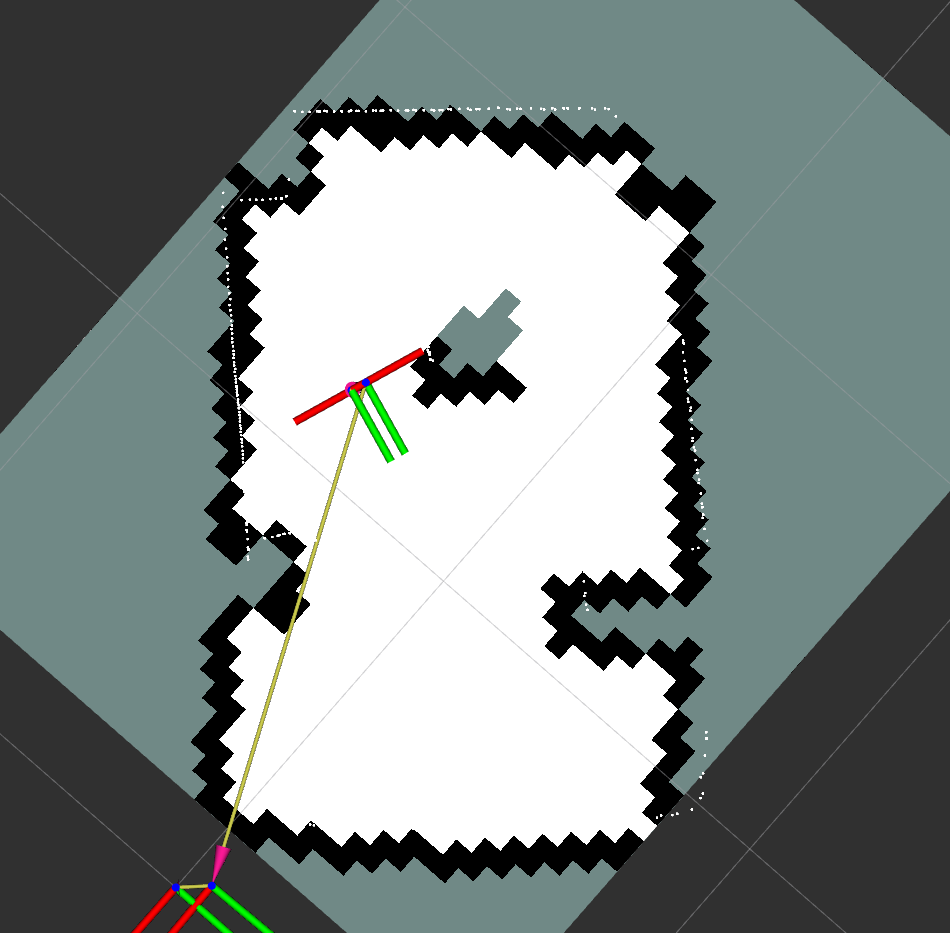
\includegraphics[width=0.8\textwidth]{images/BFS-real.png}
            \caption{BFS žemėlapis}
        \end{figure}
    \end{columns}
\end{frame}

%% 12. Rezultatai: simuliacija
\begin{frame}{Rezultatai: simuliacija}
    \begin{table}
        \centering
        \begin{tabular}{|l|c|c|c|}
            \hline
            \textbf{Algoritmas} & \textbf{Laikas (s)} & \textbf{Atstumas (m)} & \textbf{Plotas (m²)} \\
            \hline
            Frontier & 372,6 & 38,7 & 86,7 \\
            \hline
            BFS & 210,2 & 21,8 & 86,1 \\
            \hline
        \end{tabular}
    \end{table}
    
    \begin{columns}[onlytextwidth]
        \column{0.5\textwidth}
        \begin{figure}
            \centering
            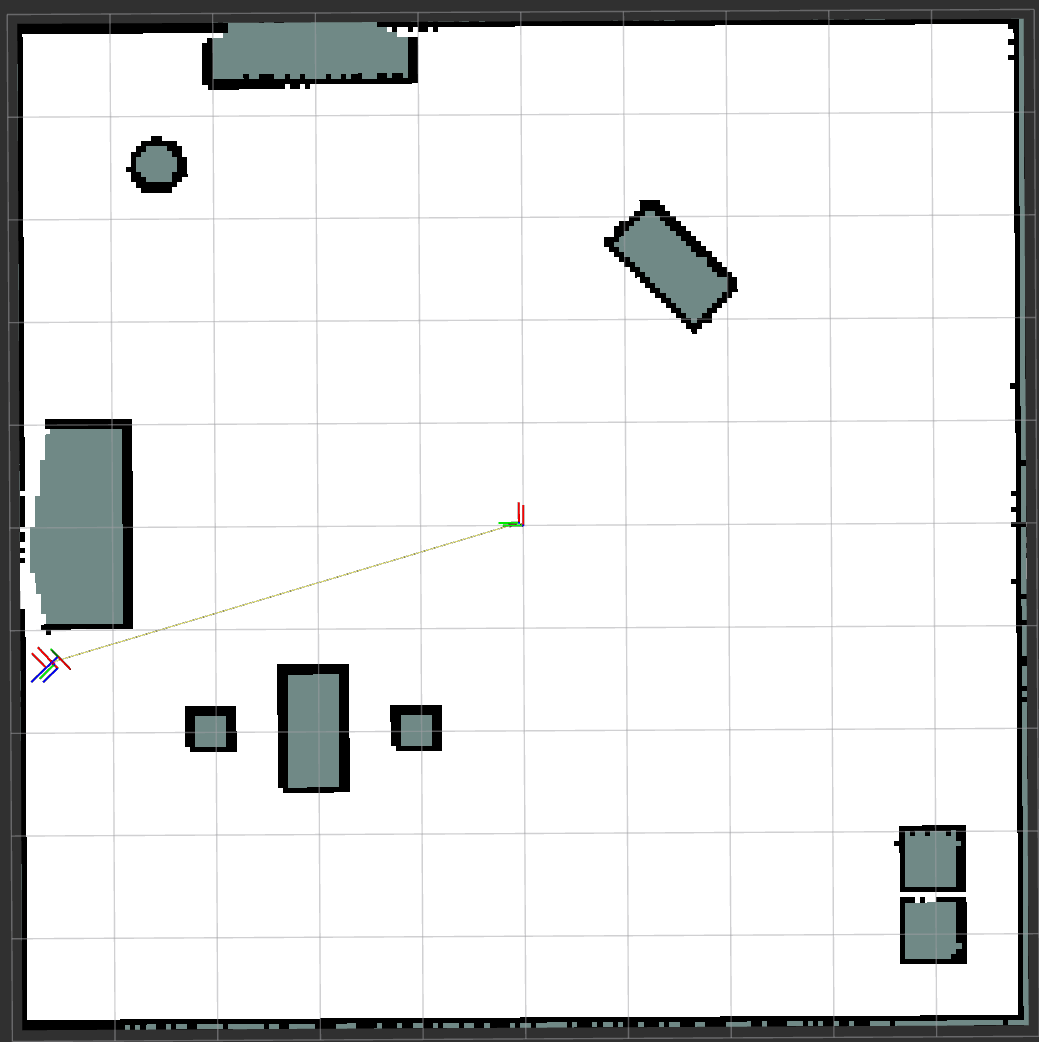
\includegraphics[width=0.8\textwidth]{images/frontier-sim.png}
            \caption{Frontier žemėlapis}
        \end{figure}
        \column{0.5\textwidth}
        \begin{figure}
            \centering
            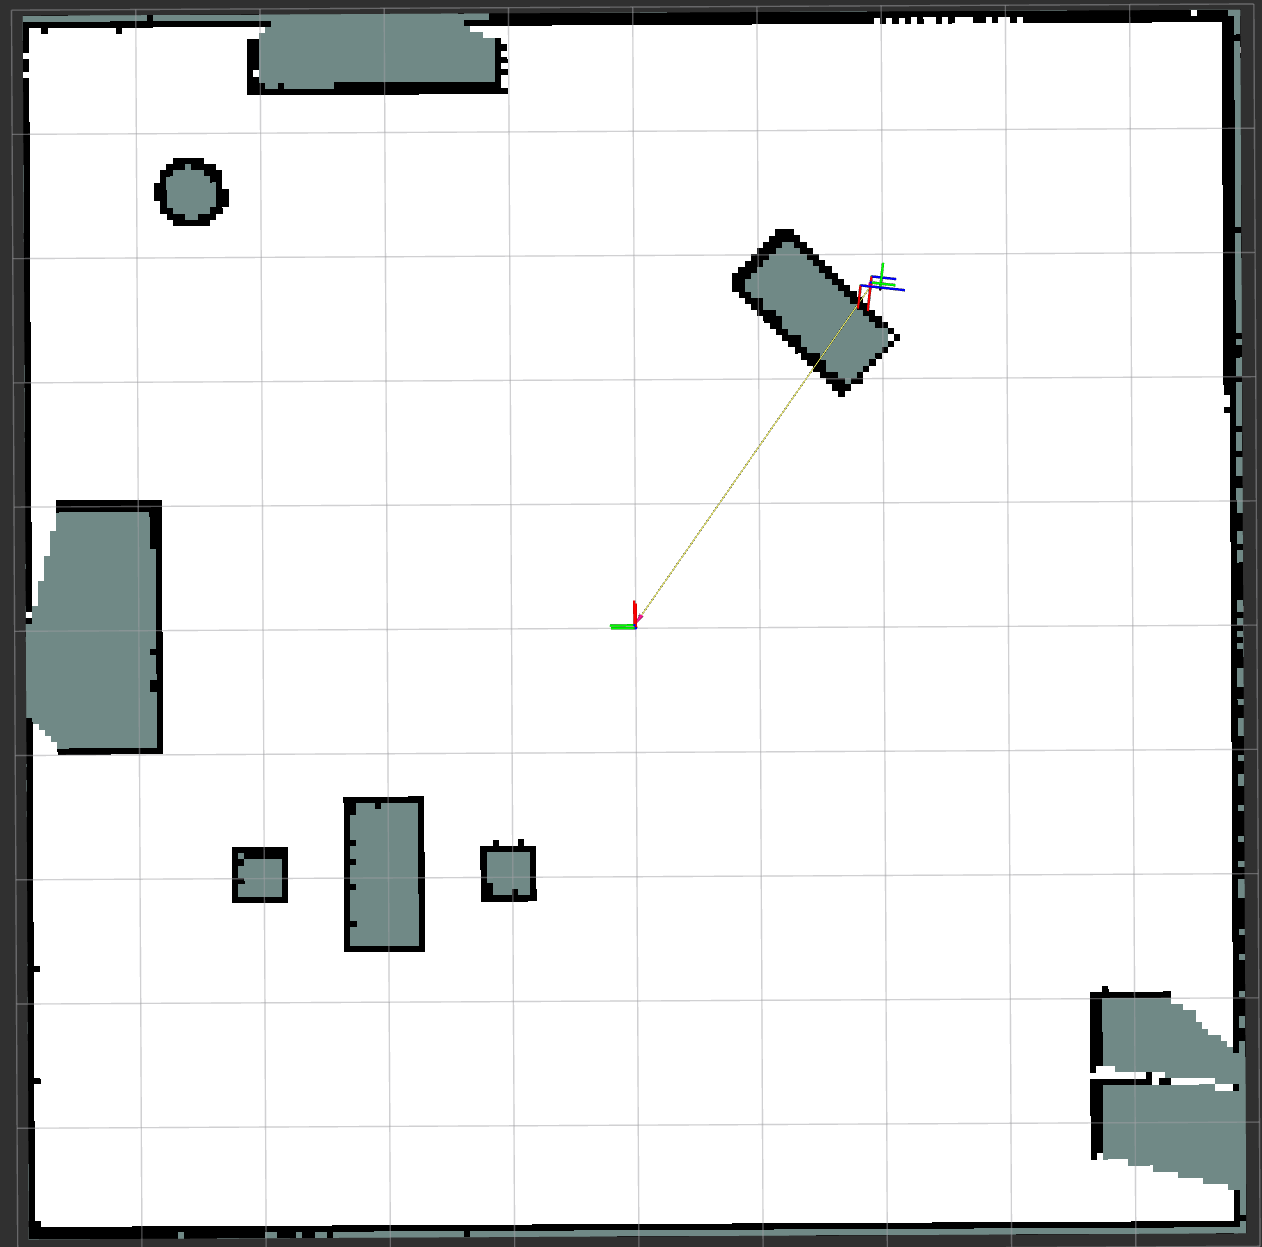
\includegraphics[width=0.8\textwidth]{images/BFS-sim.png}
            \caption{BFS žemėlapis}
        \end{figure}
    \end{columns}
\end{frame}

%% 13. Išvados
\begin{frame}{Išvados}
    \begin{enumerate}
        \item Atlikta literatūros analizė leido apibrėžti autonominio tyrinėjimo ir SLAM principus
        \item Paruošta fizinė roboto sistema, užtikrinanti patikimą jutiklių ir pavarų veikimą
        \item Sukurta simuliacinė aplinka sudarė sąlygas testuoti ir palyginti algoritmus
        \item Realizuoti \textbf{Frontier} ir \textbf{BFS} algoritmai, leidę autonomiškai tirti aplinką
        \item Palyginti \textbf{Frontier} ir \textbf{BFS} algoritmai ir aptarti jų skirtumai
        \item Realioje aplinkoje algoritmų veikimą reikšmingai veikia fiziniai apribojimai, neatsispindintys simuliacijoje
    \end{enumerate}
\end{frame}

%% 14. Klausimai
\begin{frame}
    \begin{center}
        \Huge Ačiū už dėmesį
    \end{center}
\end{frame}

\end{document}
